\subsection{Outliers and influential observations}
For each of the locations figures \ref{fig3a_temp} and \ref{fig3a_pressure} show the leverage of the data points plotted against temperature and air pressure, respectively (for the model that uses the temperature, location and pressure features as well as the interaction between temperature and pressure). Notably, the leverages are significantly higher for the measurments in Abisko and Lund than in Uppsala. This is perhaps not surprising as there are more measurements in Uppsala than in any of the other regions, meaning that Abisko and Lund are outliers in the region feature space. 

\begin{figure}[H]
\centering
	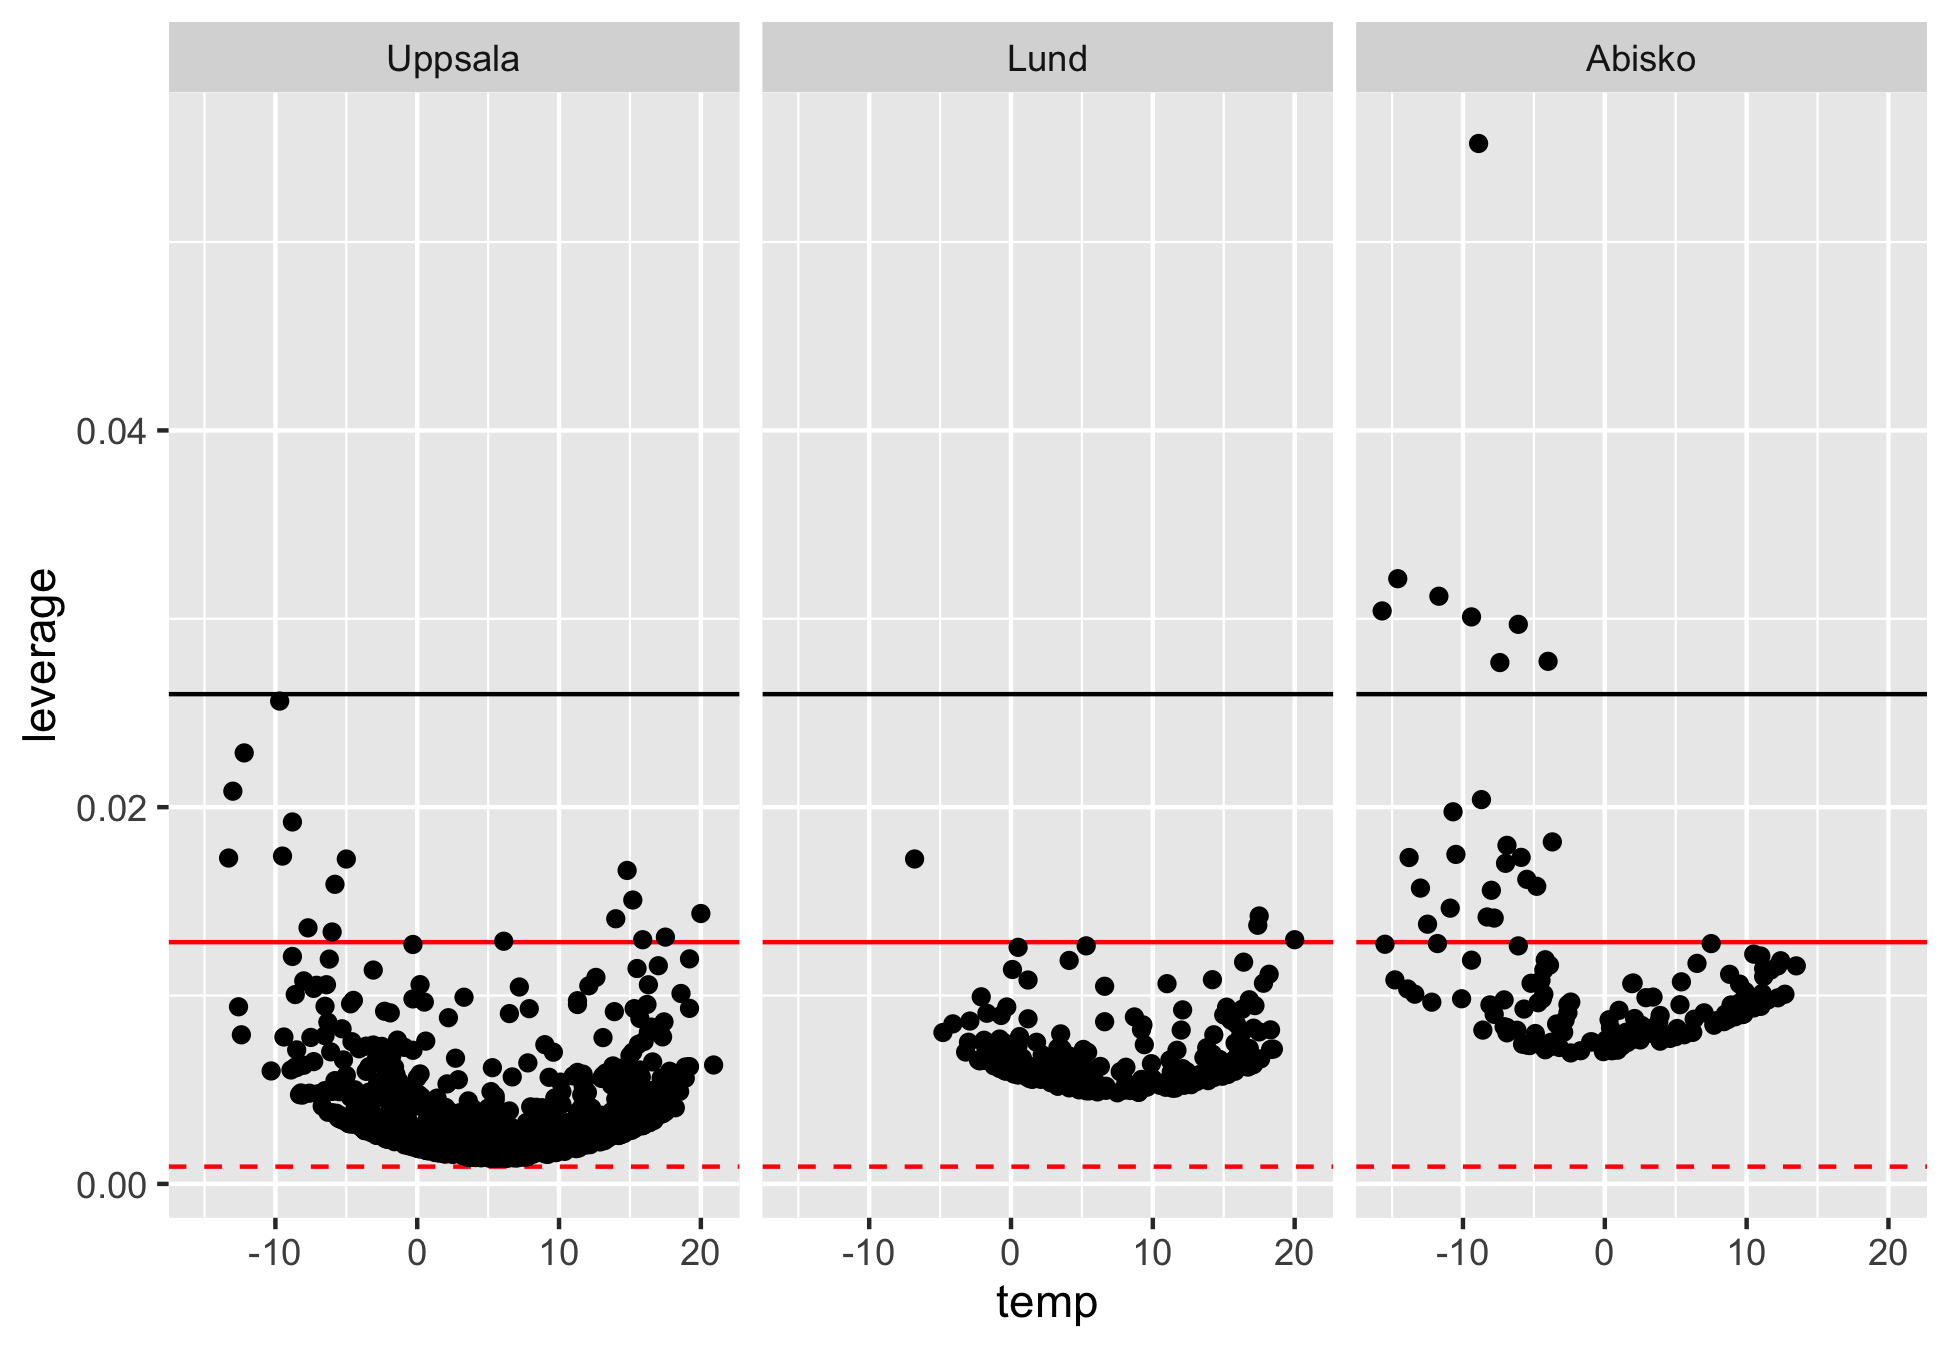
\includegraphics[width=0.7\textwidth]{Mallen/Allt/Figures/fig3a_temp.png}    		\caption{Data point leverage plotted against temperature, for each of the three locations. Points above the black lines have leverages over 0.026  }
    \label{fig3a_temp}
\end{figure}


\begin{figure}[H]
\centering
	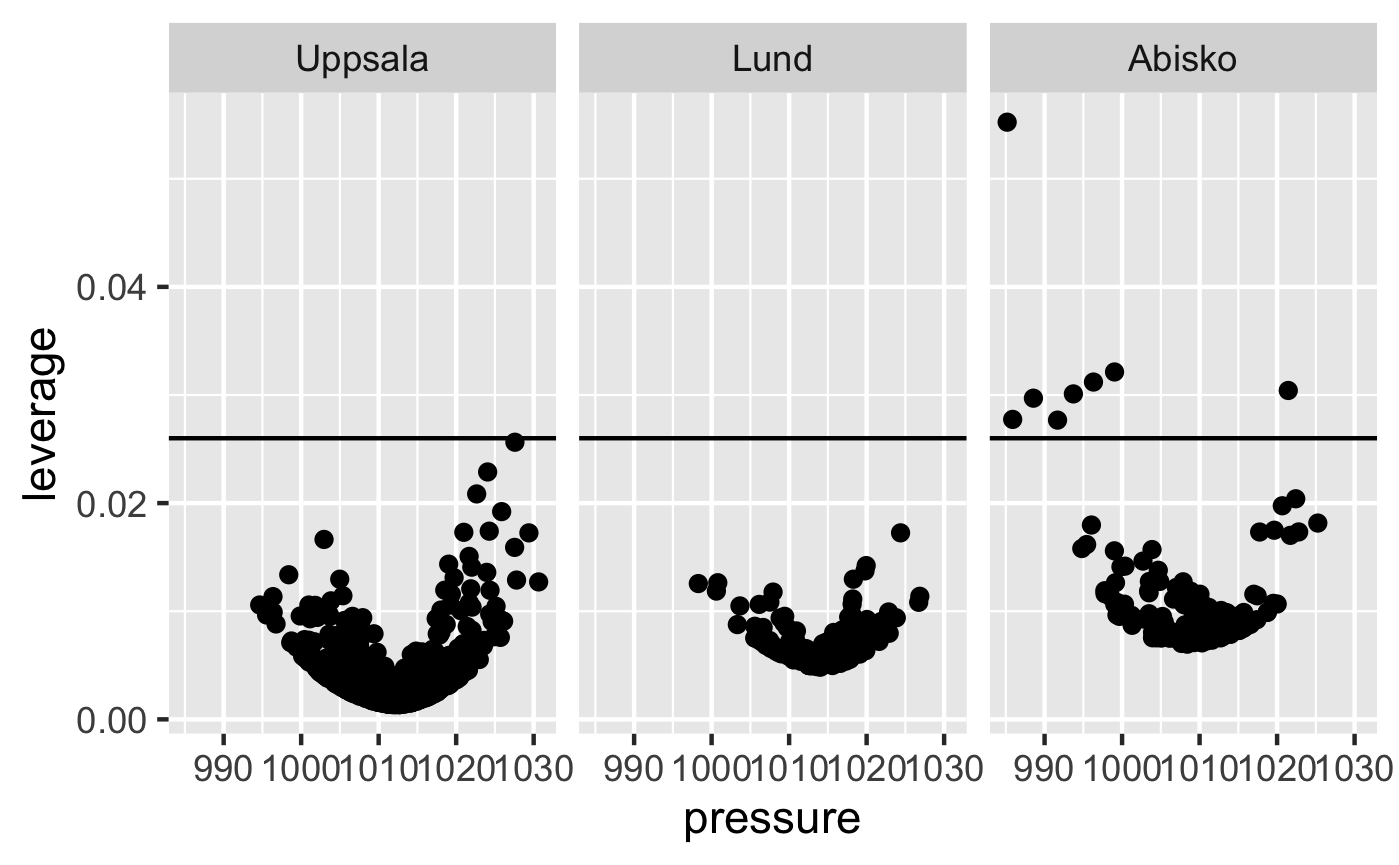
\includegraphics[width=0.8\textwidth]{Mallen/Allt/Figures/fig3a_pressure.png}    		\caption{Data point leverage plotted against temperature, for each of the three locations. Points above the black lines have leverages over 0.026 }
    \label{fig3a_pressure}
\end{figure}
Figure \ref{fig3b} below shows temperature plotted against air pressure for the data points, separately for each location. The data points with leverage above 0.026 (the points above the line in figures \ref{fig3a_temp} and \ref{fig3a_pressure}) were identified and are displayed in a different color than the rest. Apparently at least three factors have contributed to the high leverage in these points. Firstly, they are all measured in Abisko. Secondly, most of them have both air pressures and temperature on the low end of the spectrum. The exception is the point with a rather high pressure, but the lowest measures temperature of all points. 
\begin{figure}[H]
\centering
	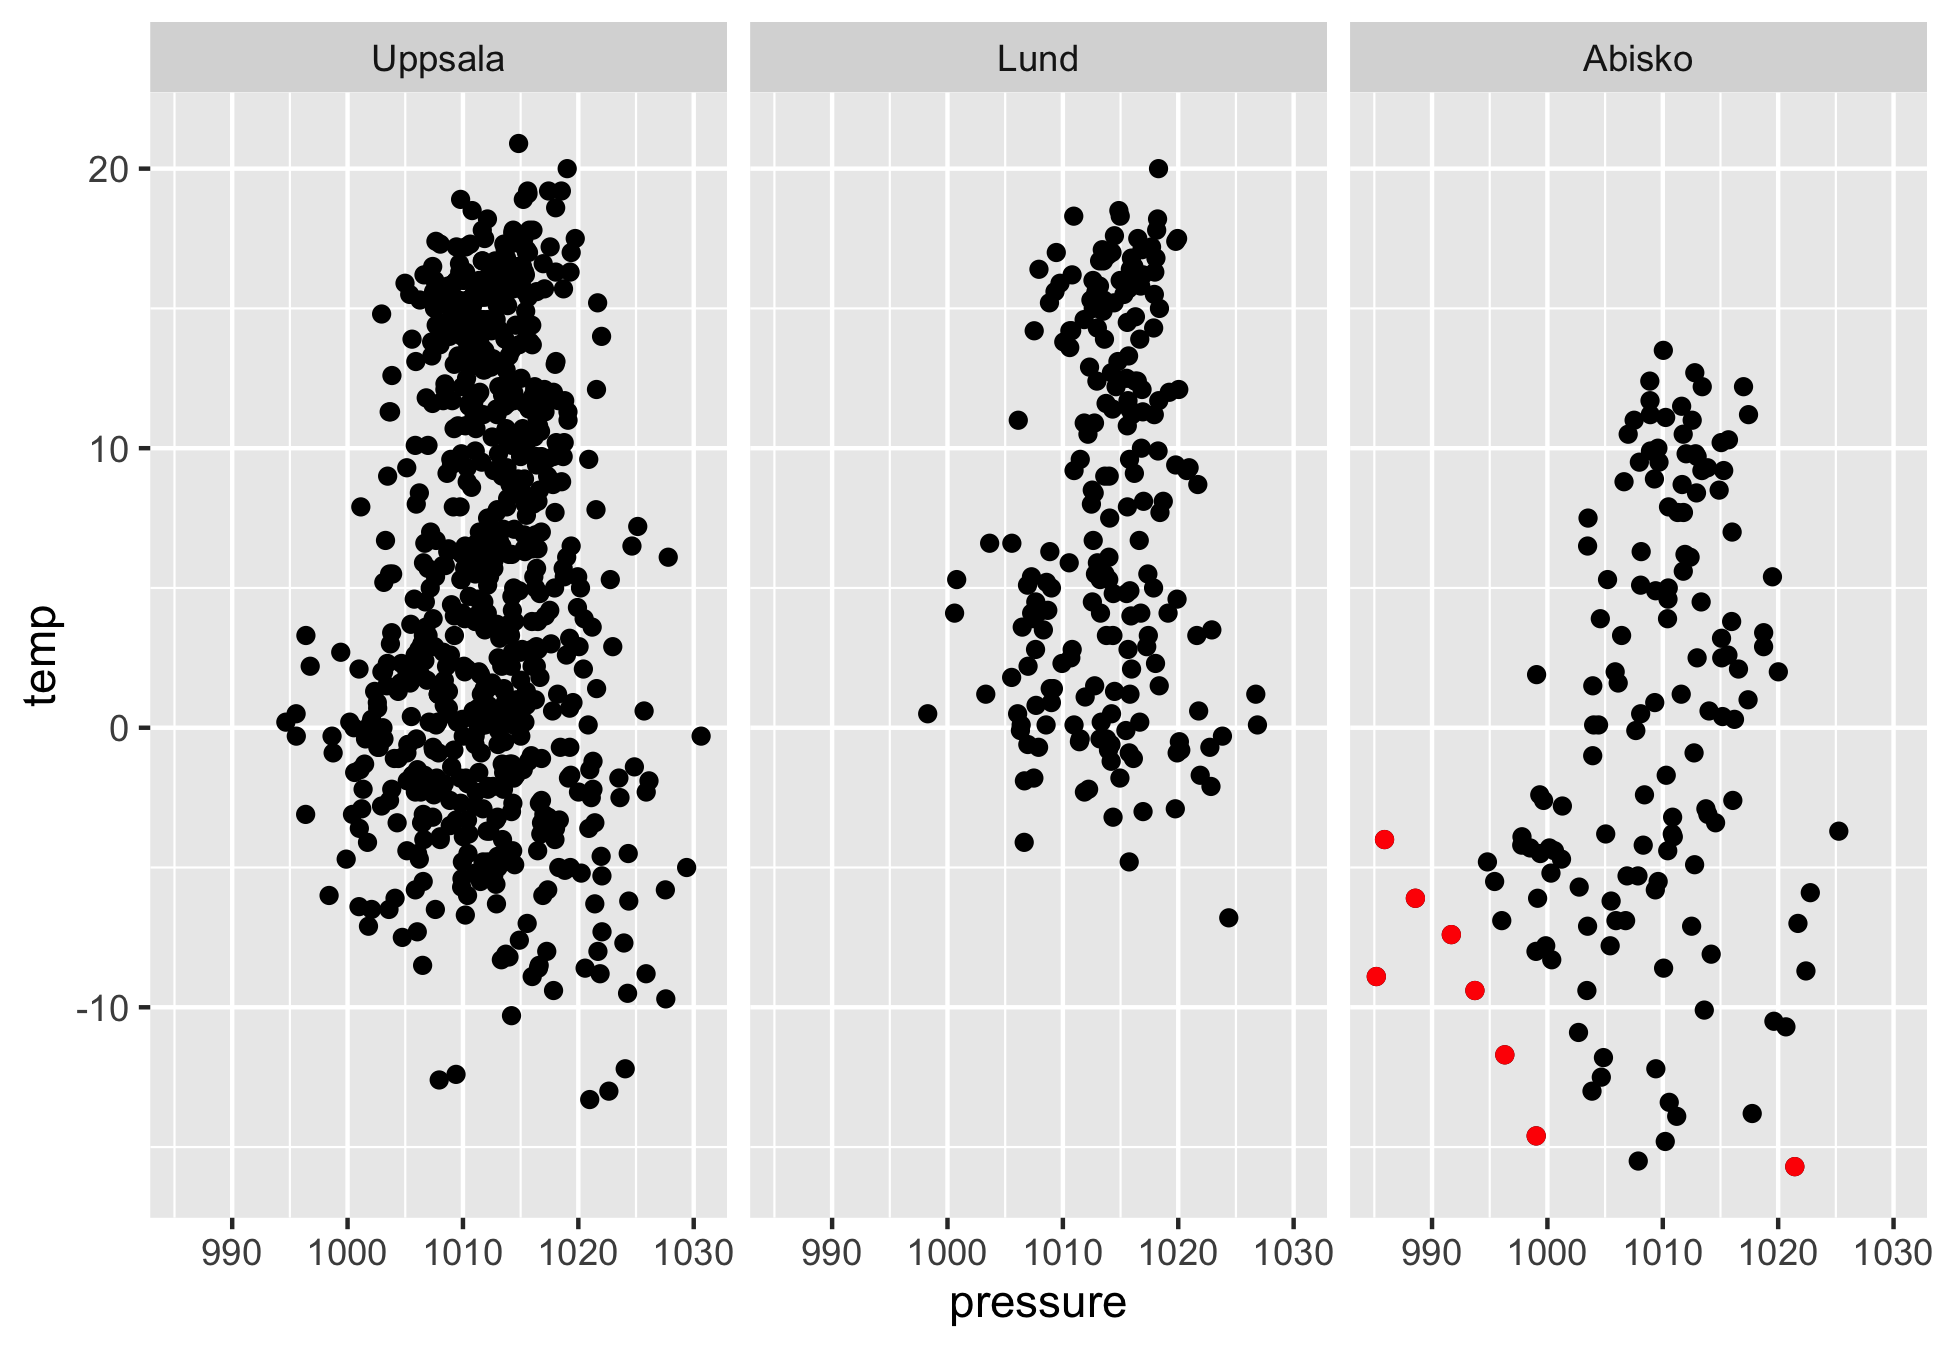
\includegraphics[width=0.8\textwidth]{Mallen/Allt/Figures/fig3b.png}    		\caption{Temperature plotted against pressure for each of the locations}
    \label{fig3b}
\end{figure}

In figure \ref{fig3c} below, the studentized residuals of the data set are plotted against the predicted values from the model using the temperature, pressure and location features as well as the interaction between temperature and pressure. The identified points with high leverage are still shown in a different color from the red ones. As is apparent from the figure, most of the points with high leverage do not have unreasonably large residuals as compared with the rest of the data. This could be because the observations are in line with the rest of the data and the model, in which case we have no problem. But it could also be because the points have influenced the fitted parameters to the extent that the predictions are heavily biased by these influential points - in this case they should probably be removed or investigated more thoroughly.

From figure \ref{fig3c} it is also apparent that there is one huge residual for an observation in Uppsala, and several other quite large residuals. Another point that should be made is that a suspiciously large proportion of the residuals are outside of the interval $\pm 2$, or even $\pm 3$. If our assumptions of normally distributed errors are true, these residuals would be \textit{highly} unlikely. The residual distribution does not seem to be centered around 0 either, but rather around a value slightly below 0. This indicates that the model predictions are generally to high. 

\begin{figure}[H]
\centering
	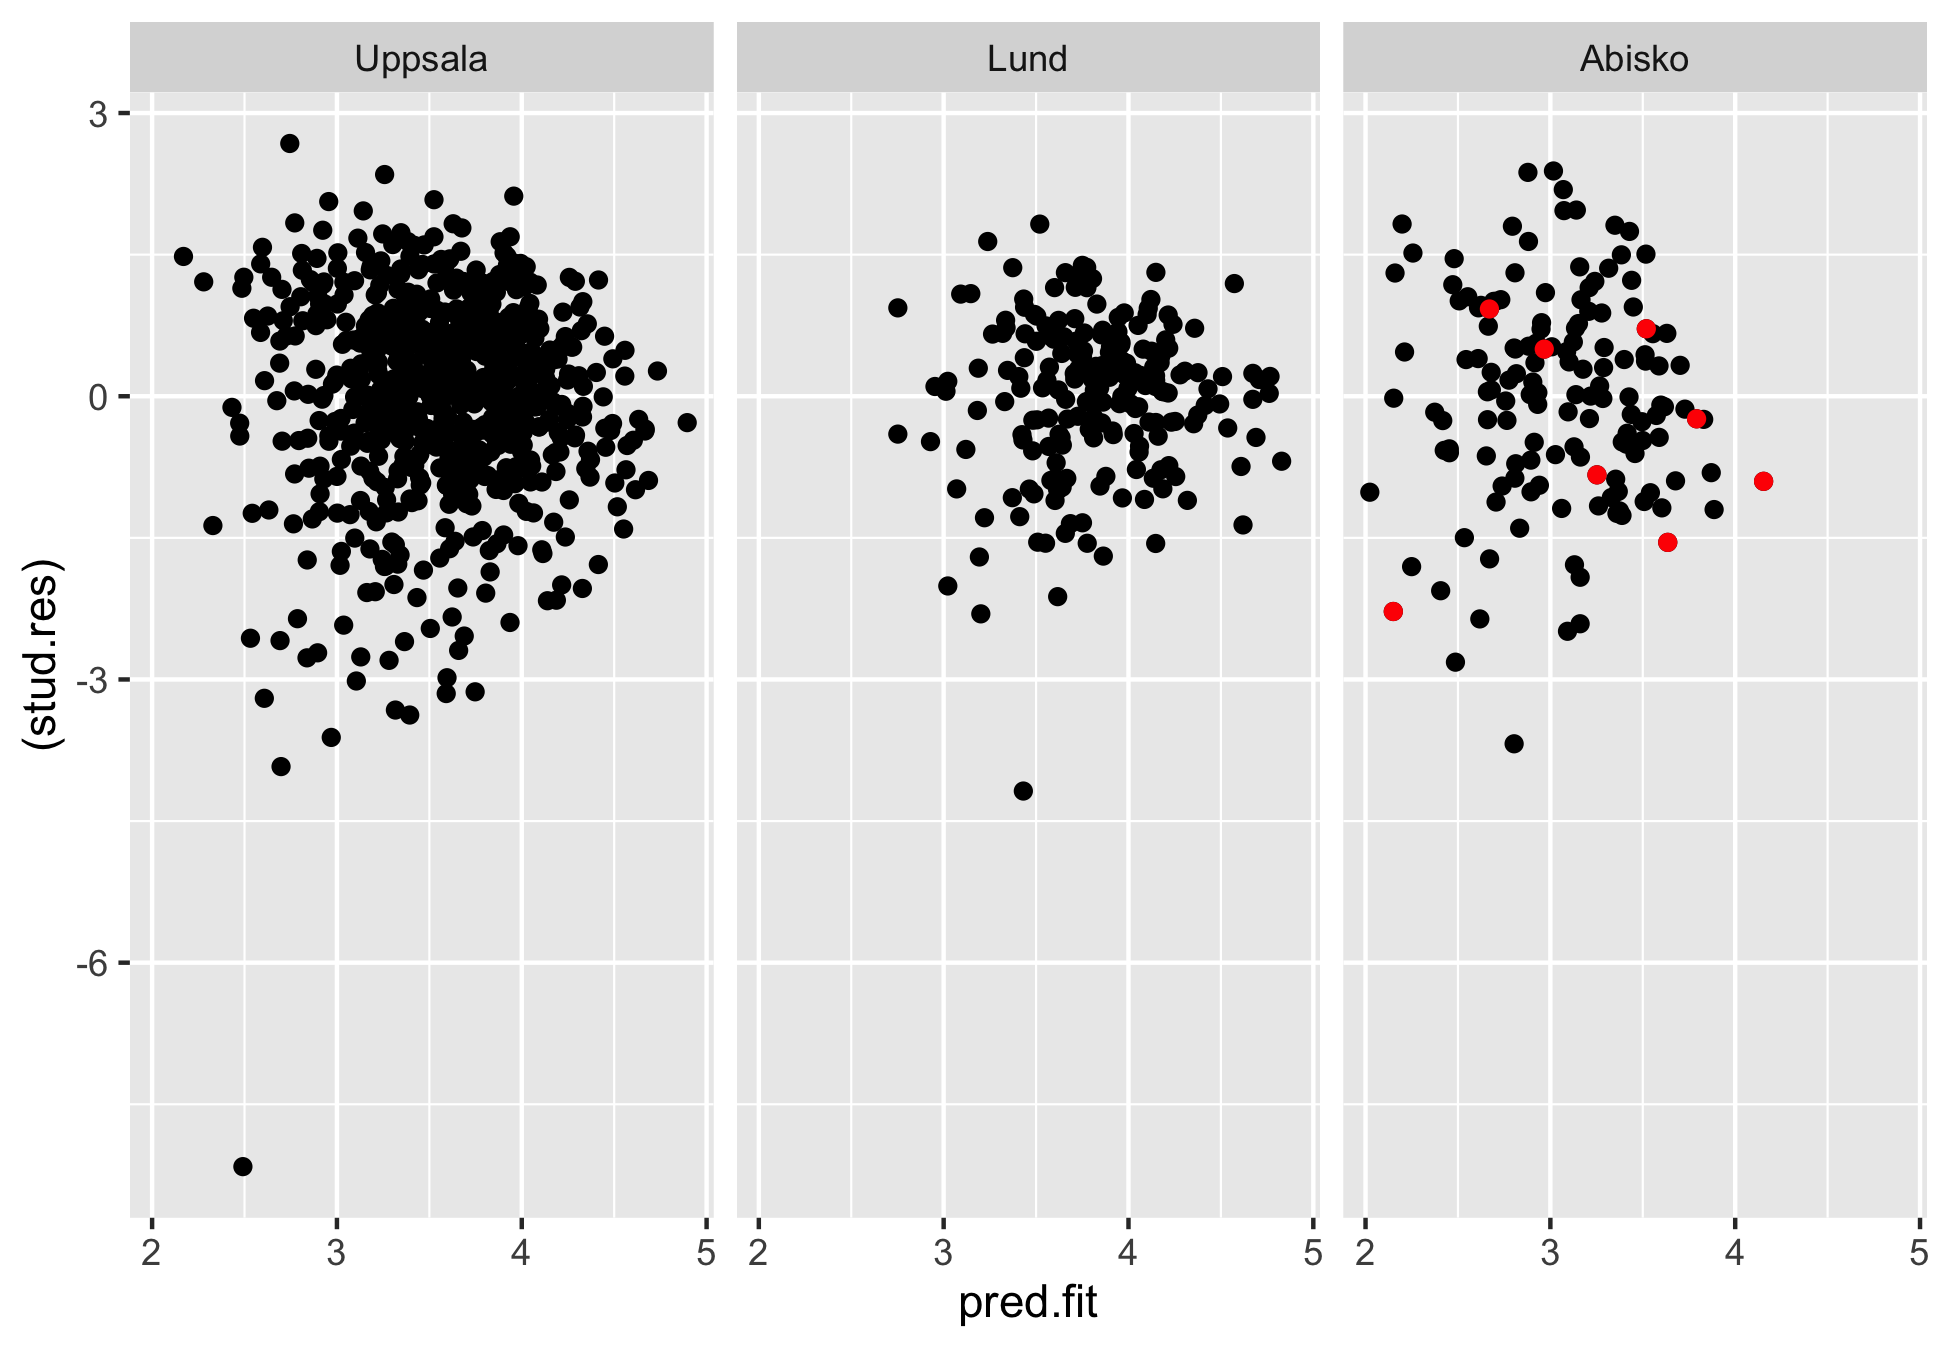
\includegraphics[width=0.8\textwidth]{Mallen/Allt/Figures/fig3c.png}    		\caption{Temperature plotted against pressure for each of the locations}
    \label{fig3c}
\end{figure}

Below (figures \ref{fig3c_pressure} and \ref{fig3c_temp}) is the log-precipitation plotted against pressure and temperature, respectively. The points with the highest residuals (from figure \ref{fig3c}) for each location are highlighted in green. It is clear that these points do not seem to follow the general linear trend, especially not the points in Uppsala and Lund. Moreover, we see that most of the points highlighted in red (the ones with high leverage) seem a bit off from the linear trend of the air pressure dependence. Also, the points do not seem to be normally distributed. For the measurements in Uppsala, there seems to be a larger spread of the points below the "main cluster" than above - this observation is in line with the fact that the residuals in general seem to be slightly below 0. 

\begin{figure}[H]
\centering
	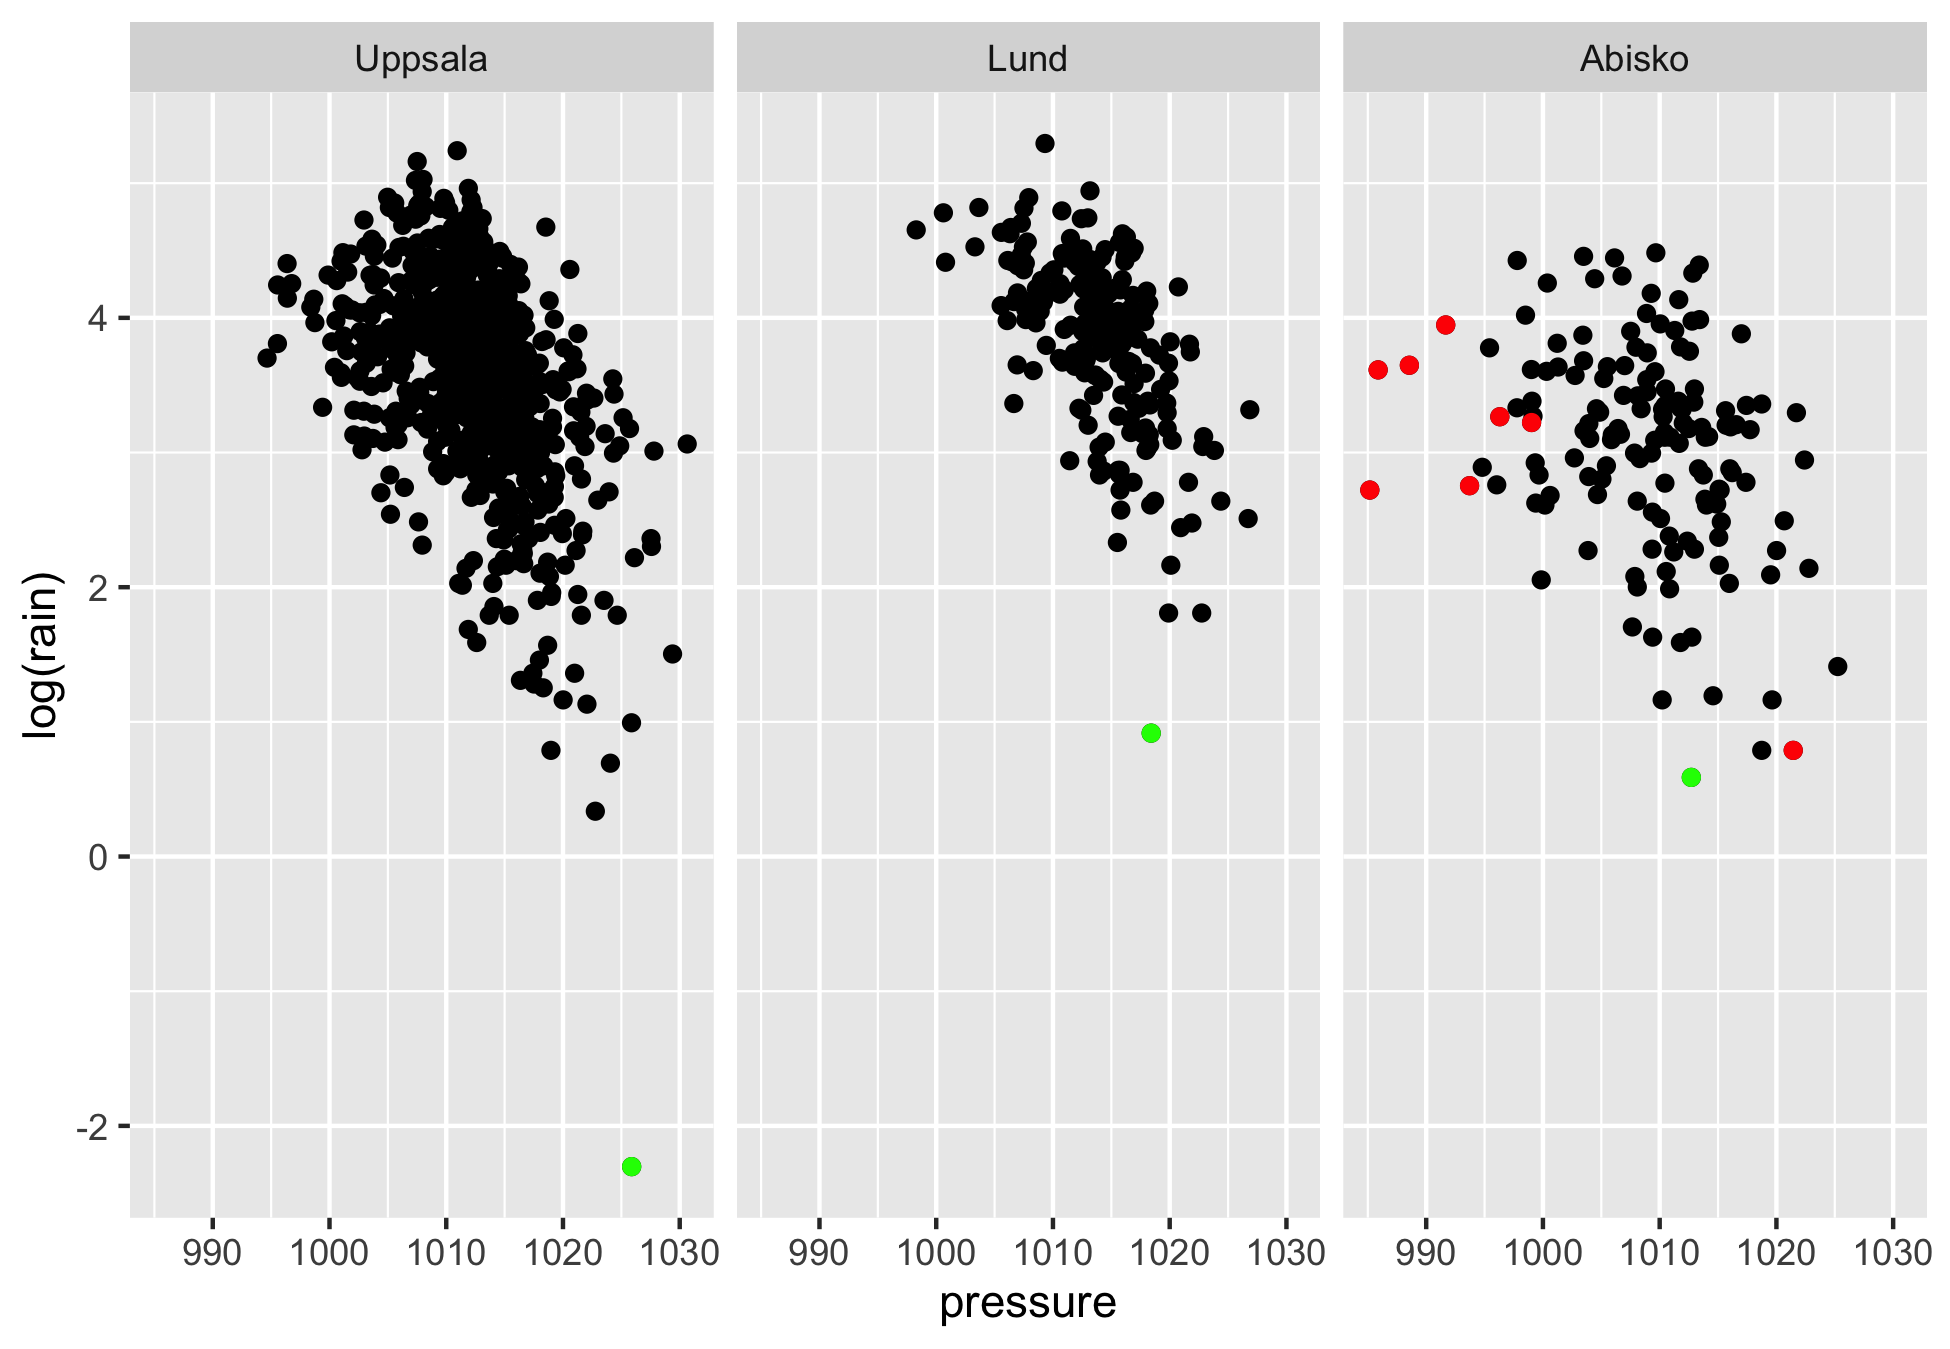
\includegraphics[width=0.8\textwidth]{Mallen/Allt/Figures/fig3c_pressure.png}    		\caption{Log-precipitation plotted against pressure for each of the locations. Green points represent the largest residuals for each location, and red points represent points with leverage above 0.026.}
    \label{fig3c_pressure}
\end{figure}

\begin{figure}[H]
\centering
	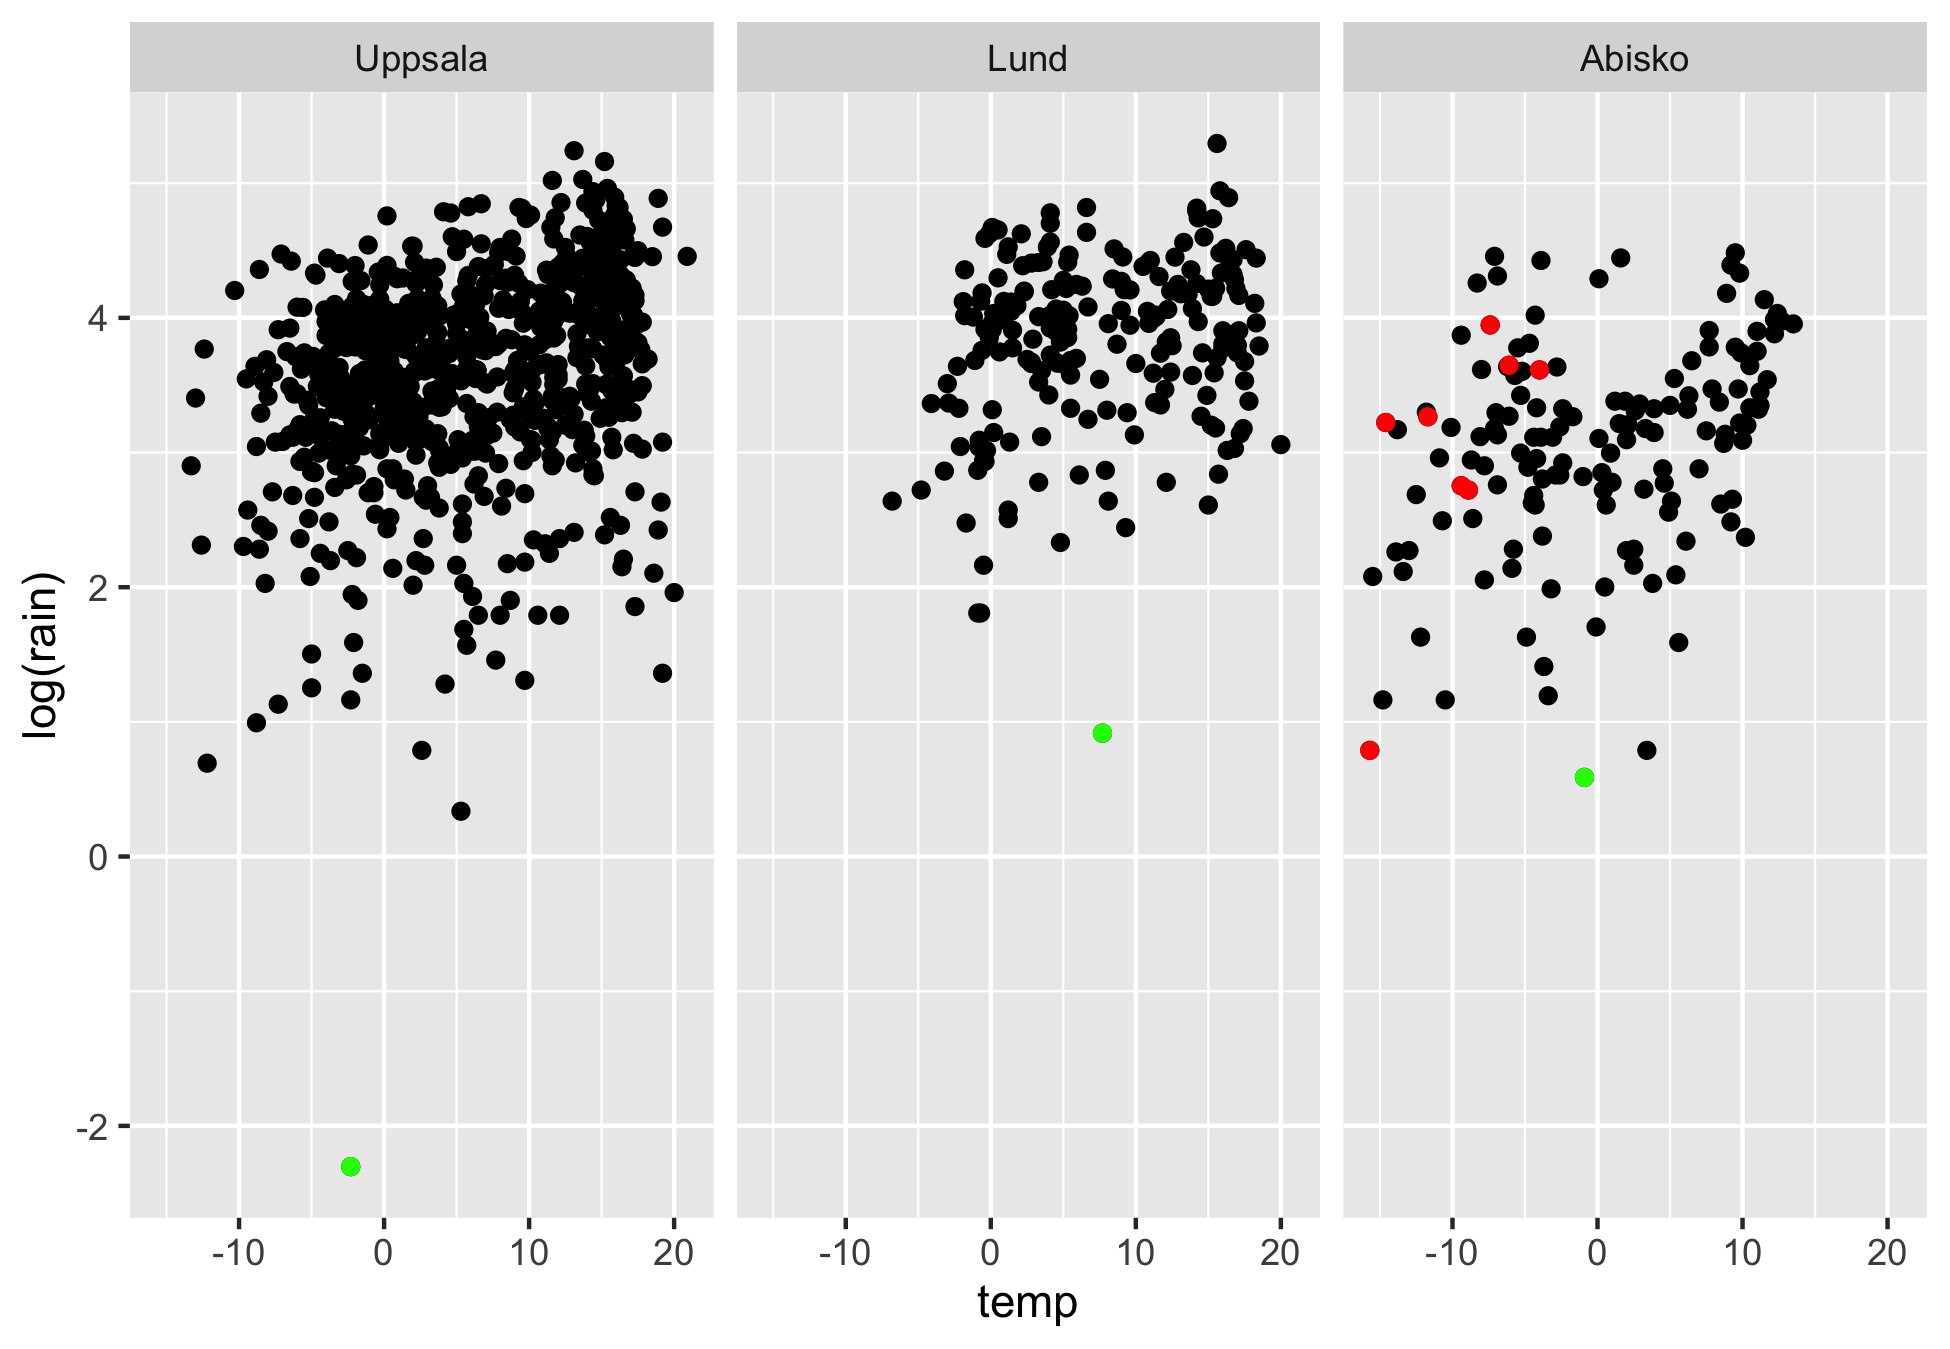
\includegraphics[width=0.8\textwidth]{Mallen/Allt/Figures/fig3c_temp.png}    		\caption{Log-precipitation plotted against temperature for each of the locations. Green points represent the largest residuals for each location, and red points represent points with leverage above 0.026.}
    \label{fig3c_temp}
\end{figure}

Figure \ref{fig3e} shows Cook's distance plotted against the temperature. We see that the points with large residuals identified previously all have had a large impact on the parameter estimates (the one in Uppsala had a huge impact). Furthermore, some of the points with high leverage had a large impact on the estimates, as well as some previously unidentified points.  
\begin{figure}[H]
\centering
	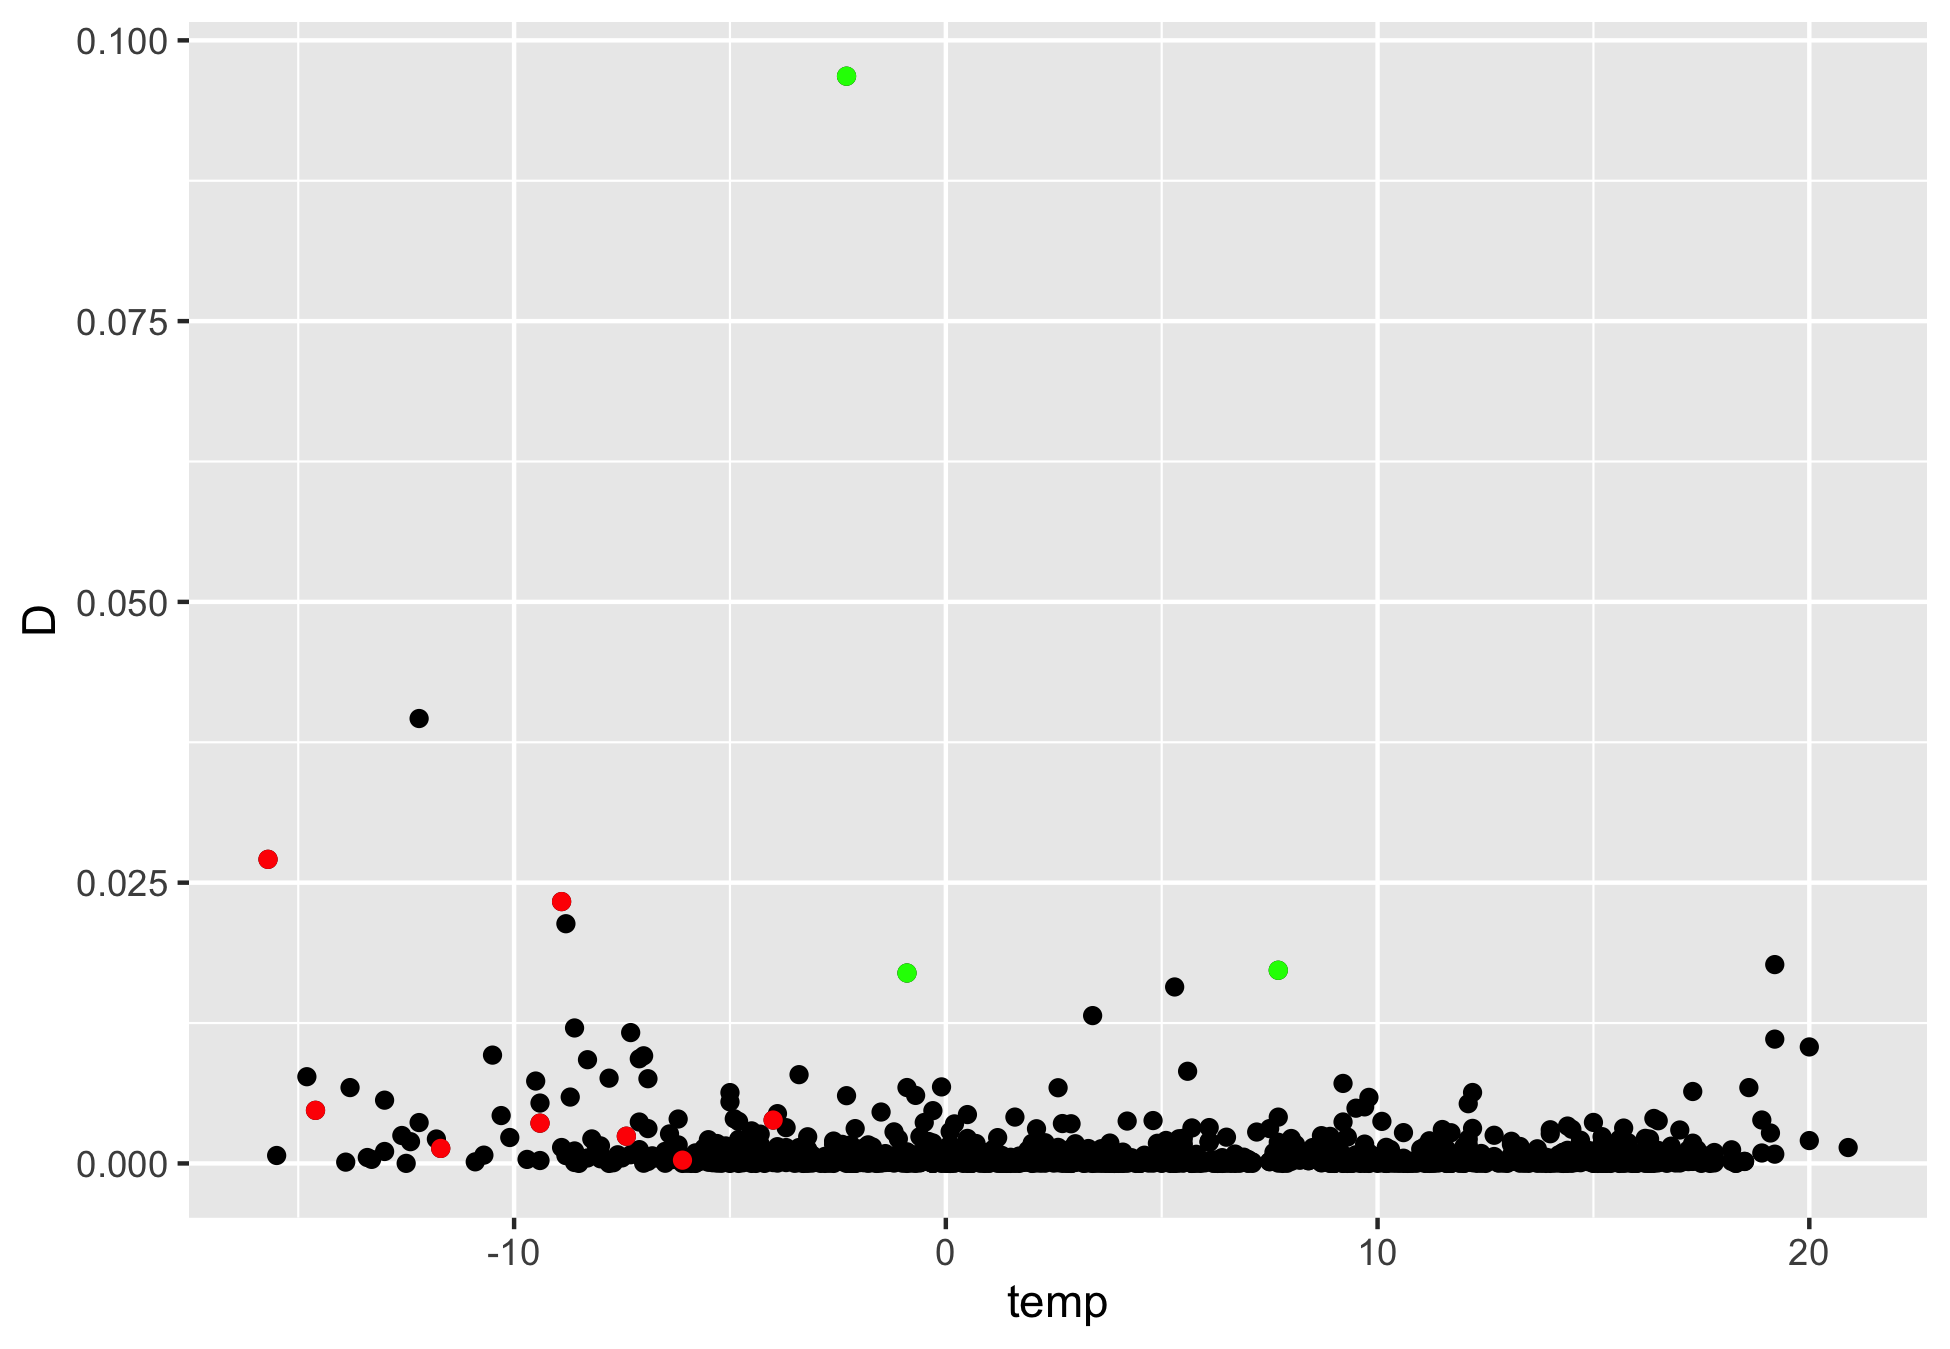
\includegraphics[width=0.8\textwidth]{Mallen/Allt/Figures/fig3e.png}    		\caption{Cook's D plotted against temperature.}
    \label{fig3e}
\end{figure}

The model was refitted using all previous data points except some. The data points that were excluded were the three points with the highest residuals for each location, and all points with larger Cook's D than these. The studentized residuals and Cook's D of the refitted model are shown in figure \ref{fig3f_res} and \ref{fig3f_D}, respectively. These look better than the corresponding graphs in figures \ref{fig3c} and \ref{fig3e}, but still not totally convincing. For one thing, the variance of the residuals seem higher for lower predicted values. Additionally, the variance does not appear to be constant for all locations (this could in part be explained by the fact that there are more observations in Uppsala though).

\begin{figure}[H]
\centering
	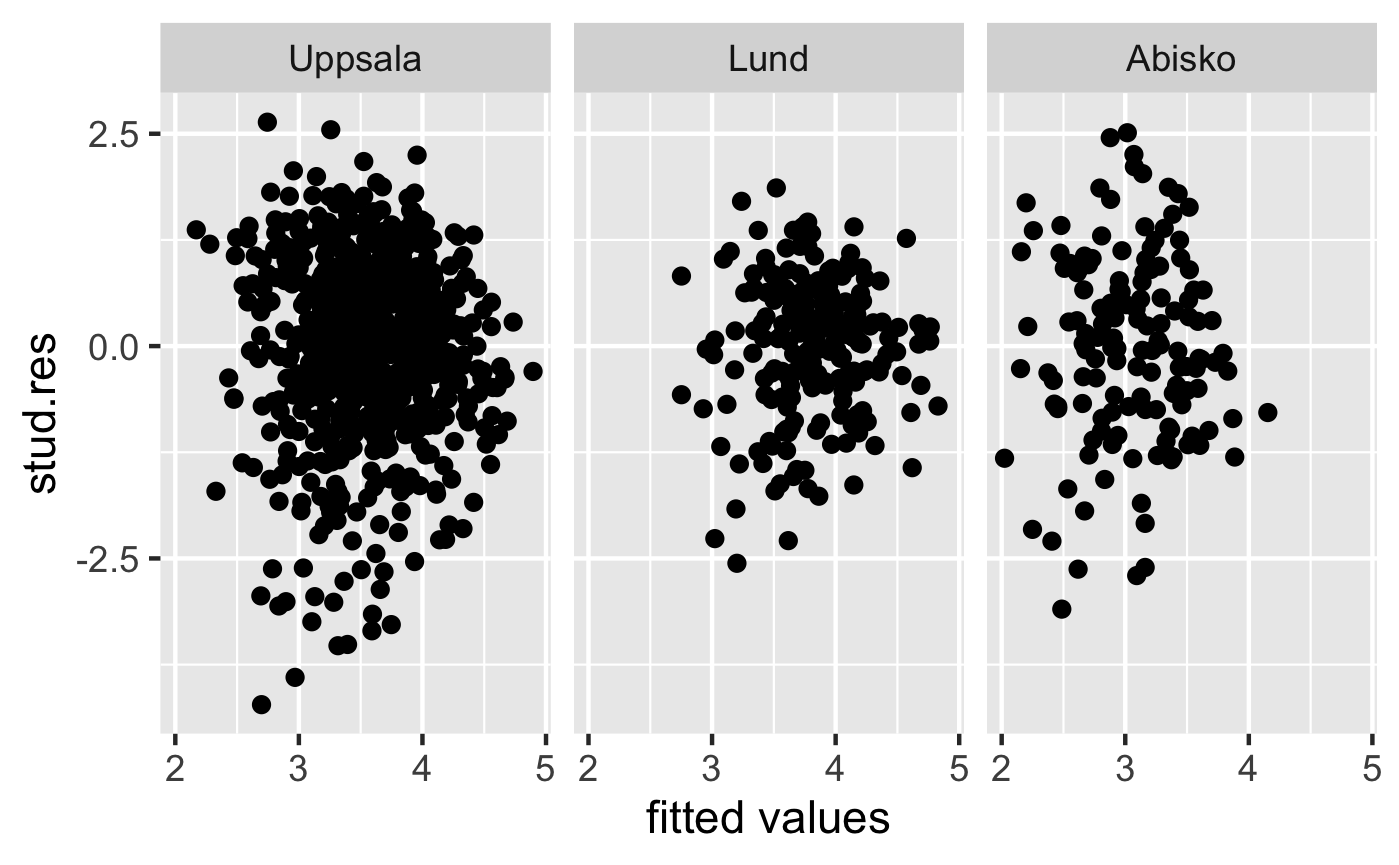
\includegraphics[width=0.8\textwidth]{Mallen/Allt/Figures/fig3f_res.png}    		\caption{Log-precipitation plotted against temperature for each of the locations. Green points represent the largest residuals for each location, and red points represent points with leverage above 0.026.}
    \label{fig3f_res}
\end{figure}

\begin{figure}[H]
\centering
	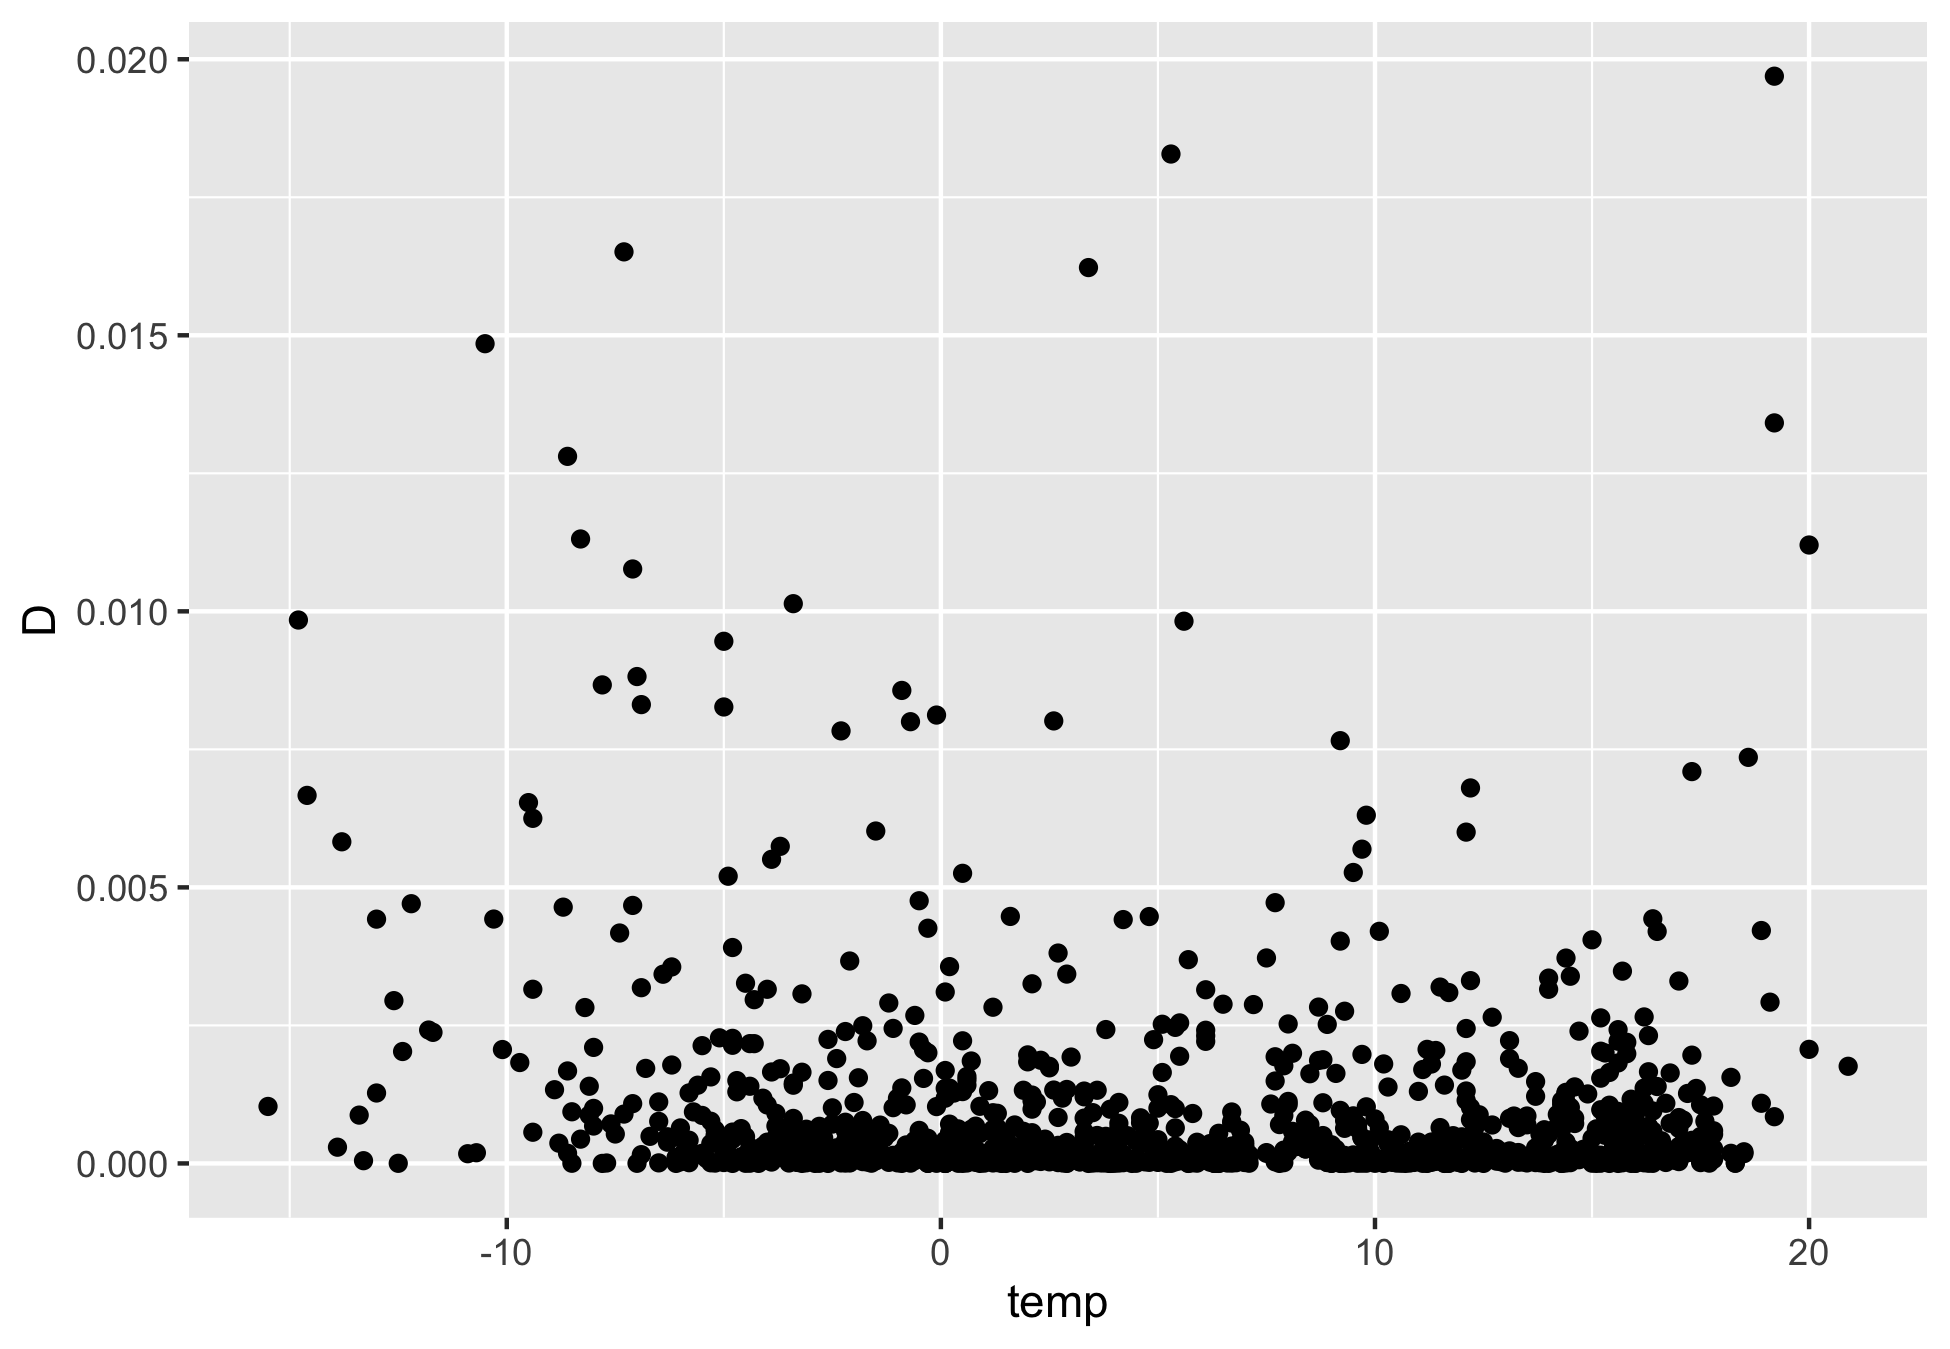
\includegraphics[width=0.8\textwidth]{Mallen/Allt/Figures/fig3f_D.png}    		\caption{Log-precipitation plotted against temperature for each of the locations. Green points represent the largest residuals for each location, and red points represent points with leverage above 0.026.}
    \label{fig3f_D}
\end{figure}

\subsection{Model comparisons}

All previously discussed models were refitted with the new data set (i.e. the one with fewer points). For each of the models the $R^2$ and adjusted $R^2$ scores were calculated as well as the AIC and BIC scores. The result is given in table \ref{resulttable}. Both the AIC and the BIC scores indicate that the biggest model is the best, and the adjusted $R^2$ score tells us that almost $40\%$ of the variability in the sample is explained by the model. 
\begin{table}[H]
\centering
\begin{tabular}{|
>{\columncolor[HTML]{FFFFFF}}l |
>{\columncolor[HTML]{FFFFFF}}l |
>{\columncolor[HTML]{FFFFFF}}l |
>{\columncolor[HTML]{FFFFFF}}l |
>{\columncolor[HTML]{FFFFFF}}l |}
\hline
Model parameters                  & $R^2$     & $R^2_{adj}$ & AIC      & BIC      \\ \hline
Temperature                       & 0.1106402 & 0.1098235   & 2434.717 & 2449.702 \\ \hline
Temperature + Pressure            & 0.2877870 & 0.2864778   & 2194.379 & 2214.359 \\ \hline
Temperature * Pressure            & 0.3161416 & 0.3142543   & 2152.056 & 2177.030 \\ \hline
Temperature * Pressure + Location & 0.3980373 & 0.3952453   & 1884.574 & 1919.493 \\ \hline
\end{tabular}
\caption{Scores for the different models, refitted with smaller data set.}
\label{resulttable}
\end{table}
A new model was fitted, where interaction terms between all other features were added. This new model was to the previous best one with a partial F-test and the P-value calculated to be 0.2989. This means that none of the newly added interaction terms differ significantly from 0.

Backward and forward selections between the last model and the first one both ended up in the model that performed best according to table \ref{resulttable}. However, when seasons where added as a possible parameter, a forward selection procedure ended up in a different model, namely one using 5 different parameters: temperature, pressure, location, season and the interaction term between temperature and pressure, indicating that there in fact is a seasonal difference in precipitation. This final model managed to achive an adjusted $R^2$ score of 0.4241668, meaning it explains slightly more than 42\% of the variability in the data. 